% Options for packages loaded elsewhere
\PassOptionsToPackage{unicode}{hyperref}
\PassOptionsToPackage{hyphens}{url}
%
\documentclass[
]{article}
\usepackage{amsmath,amssymb}
\usepackage{lmodern}
\usepackage{iftex}
\ifPDFTeX
  \usepackage[T1]{fontenc}
  \usepackage[utf8]{inputenc}
  \usepackage{textcomp} % provide euro and other symbols
\else % if luatex or xetex
  \usepackage{unicode-math}
  \defaultfontfeatures{Scale=MatchLowercase}
  \defaultfontfeatures[\rmfamily]{Ligatures=TeX,Scale=1}
\fi
% Use upquote if available, for straight quotes in verbatim environments
\IfFileExists{upquote.sty}{\usepackage{upquote}}{}
\IfFileExists{microtype.sty}{% use microtype if available
  \usepackage[]{microtype}
  \UseMicrotypeSet[protrusion]{basicmath} % disable protrusion for tt fonts
}{}
\makeatletter
\@ifundefined{KOMAClassName}{% if non-KOMA class
  \IfFileExists{parskip.sty}{%
    \usepackage{parskip}
  }{% else
    \setlength{\parindent}{0pt}
    \setlength{\parskip}{6pt plus 2pt minus 1pt}}
}{% if KOMA class
  \KOMAoptions{parskip=half}}
\makeatother
\usepackage{xcolor}
\usepackage{color}
\usepackage{fancyvrb}
\newcommand{\VerbBar}{|}
\newcommand{\VERB}{\Verb[commandchars=\\\{\}]}
\DefineVerbatimEnvironment{Highlighting}{Verbatim}{commandchars=\\\{\}}
% Add ',fontsize=\small' for more characters per line
\newenvironment{Shaded}{}{}
\newcommand{\AlertTok}[1]{\textcolor[rgb]{1.00,0.00,0.00}{\textbf{#1}}}
\newcommand{\AnnotationTok}[1]{\textcolor[rgb]{0.38,0.63,0.69}{\textbf{\textit{#1}}}}
\newcommand{\AttributeTok}[1]{\textcolor[rgb]{0.49,0.56,0.16}{#1}}
\newcommand{\BaseNTok}[1]{\textcolor[rgb]{0.25,0.63,0.44}{#1}}
\newcommand{\BuiltInTok}[1]{#1}
\newcommand{\CharTok}[1]{\textcolor[rgb]{0.25,0.44,0.63}{#1}}
\newcommand{\CommentTok}[1]{\textcolor[rgb]{0.38,0.63,0.69}{\textit{#1}}}
\newcommand{\CommentVarTok}[1]{\textcolor[rgb]{0.38,0.63,0.69}{\textbf{\textit{#1}}}}
\newcommand{\ConstantTok}[1]{\textcolor[rgb]{0.53,0.00,0.00}{#1}}
\newcommand{\ControlFlowTok}[1]{\textcolor[rgb]{0.00,0.44,0.13}{\textbf{#1}}}
\newcommand{\DataTypeTok}[1]{\textcolor[rgb]{0.56,0.13,0.00}{#1}}
\newcommand{\DecValTok}[1]{\textcolor[rgb]{0.25,0.63,0.44}{#1}}
\newcommand{\DocumentationTok}[1]{\textcolor[rgb]{0.73,0.13,0.13}{\textit{#1}}}
\newcommand{\ErrorTok}[1]{\textcolor[rgb]{1.00,0.00,0.00}{\textbf{#1}}}
\newcommand{\ExtensionTok}[1]{#1}
\newcommand{\FloatTok}[1]{\textcolor[rgb]{0.25,0.63,0.44}{#1}}
\newcommand{\FunctionTok}[1]{\textcolor[rgb]{0.02,0.16,0.49}{#1}}
\newcommand{\ImportTok}[1]{#1}
\newcommand{\InformationTok}[1]{\textcolor[rgb]{0.38,0.63,0.69}{\textbf{\textit{#1}}}}
\newcommand{\KeywordTok}[1]{\textcolor[rgb]{0.00,0.44,0.13}{\textbf{#1}}}
\newcommand{\NormalTok}[1]{#1}
\newcommand{\OperatorTok}[1]{\textcolor[rgb]{0.40,0.40,0.40}{#1}}
\newcommand{\OtherTok}[1]{\textcolor[rgb]{0.00,0.44,0.13}{#1}}
\newcommand{\PreprocessorTok}[1]{\textcolor[rgb]{0.74,0.48,0.00}{#1}}
\newcommand{\RegionMarkerTok}[1]{#1}
\newcommand{\SpecialCharTok}[1]{\textcolor[rgb]{0.25,0.44,0.63}{#1}}
\newcommand{\SpecialStringTok}[1]{\textcolor[rgb]{0.73,0.40,0.53}{#1}}
\newcommand{\StringTok}[1]{\textcolor[rgb]{0.25,0.44,0.63}{#1}}
\newcommand{\VariableTok}[1]{\textcolor[rgb]{0.10,0.09,0.49}{#1}}
\newcommand{\VerbatimStringTok}[1]{\textcolor[rgb]{0.25,0.44,0.63}{#1}}
\newcommand{\WarningTok}[1]{\textcolor[rgb]{0.38,0.63,0.69}{\textbf{\textit{#1}}}}
\usepackage{graphicx}
\makeatletter
\def\maxwidth{\ifdim\Gin@nat@width>\linewidth\linewidth\else\Gin@nat@width\fi}
\def\maxheight{\ifdim\Gin@nat@height>\textheight\textheight\else\Gin@nat@height\fi}
\makeatother
% Scale images if necessary, so that they will not overflow the page
% margins by default, and it is still possible to overwrite the defaults
% using explicit options in \includegraphics[width, height, ...]{}
\setkeys{Gin}{width=\maxwidth,height=\maxheight,keepaspectratio}
% Set default figure placement to htbp
\makeatletter
\def\fps@figure{htbp}
\makeatother
\setlength{\emergencystretch}{3em} % prevent overfull lines
\providecommand{\tightlist}{%
  \setlength{\itemsep}{0pt}\setlength{\parskip}{0pt}}
\setcounter{secnumdepth}{-\maxdimen} % remove section numbering
\ifLuaTeX
  \usepackage{selnolig}  % disable illegal ligatures
\fi
\IfFileExists{bookmark.sty}{\usepackage{bookmark}}{\usepackage{hyperref}}
\IfFileExists{xurl.sty}{\usepackage{xurl}}{} % add URL line breaks if available
\urlstyle{same} % disable monospaced font for URLs
\hypersetup{
  hidelinks,
  pdfcreator={LaTeX via pandoc}}

\author{}
\date{}

\begin{document}

\hypertarget{ux43dux435ux43fux440ux435ux440ux44bux432ux43dux43eux441ux442ux44c-ux444ux443ux43dux43aux446ux438ux438-ux43cux43dux43eux433ux438ux445-ux43fux435ux440ux435ux43cux435ux43dux43dux44bux445}{%
\section{Непрерывность функции многих
переменных}\label{ux43dux435ux43fux440ux435ux440ux44bux432ux43dux43eux441ux442ux44c-ux444ux443ux43dux43aux446ux438ux438-ux43cux43dux43eux433ux438ux445-ux43fux435ux440ux435ux43cux435ux43dux43dux44bux445}}

Пусть функция \$u=f(M)\$ определена на множестве \$\{M\} \\
\textbackslash subset \textbackslash R\^{}m\$ и пусть точка
\$A\textbackslash; \textbackslash in \{M\}\$ и является \\
предельной точкой множества \$\{M\}\$.\\
Определение. Функция \$u=f(M)\$ называется \emph{непрерывной} в точке A,
если

\[\lim_{M \to A} f(M) = f(A). (9.2)\]

\emph{Точка разрыва} функции \$u=f(M)\$ - это предельная точка
множества\\
\{M\}, в которой \$f(M)\$ не является непрерывной.

\emph{Определение}. Приращением (полным приращением) функции \$u=f(M)\$
в точке A называется функция \$\textbackslash Delta u = f(M) - f(A)\$.
\\
Условие (9.2) непрерывности функции в точке A можно записать в виде:

\[\lim_{M\to A} \Delta u = \lim_{M \to A}\Bigg[ f(M) - f(A) \Bigg] = 0. (9.3)\]

Равенство (9.3) называется \emph{разностной формой условия непрерывности
функции в точке A.}\\
Пусть точки M и A имеют координаты: \$M(x\_1,...,x\_m)\$ и \\
\$A(a\_1,...,a\_m)\$. Положим \$\textbackslash Delta x\_1 = x\_1 -
a\_1,...,\textbackslash Delta x\_m = x\_m - a\_m\$, тогда \$x\_1 = a\_1
+\textbackslash Delta x\_1,...,x\_m = a\_m +\textbackslash Delta x\_m\$.

\[\Delta u = f(M)-f(A) = f(a_1,+\Delta x_1,...,a_m+\Delta x_m) - f(a_1,...,a_m).\]

Разностная форма условия непрерывности функции принимает вид

\[\lim_{\Delta x_1 \to \infty \\ ..... \\ \Delta x_m \to \infty} \Delta u=0.\]

Введем теперь понятие \emph{непрерывности функции по отдельным
переменным}.\\
Рассмотрим функцию двух переменных \$u=f(x,y)\$. Зафиксируем значение
аргумента y, положив \$y=y\_0\$(рис.9.3). Получаем функцию одной
переменной \$f(x,y\_0)\$. Если эта функция непрерывна в точке \$x\_0\$,
то есть \$\textbackslash lim\_\{x\textbackslash to x\_0\} f(x,y\_0) =
f(x\_0,y\_0)\$, то будем говорить, что функция \$u=f(x,y)\$ непрерывна в
точке \$M\_0(x\_0,y\_0)\$ по переменной x.

Аналогично определяется непрерывность функции \$f(x,y)\$ в точке
\$M\_0\$ по переменной \$y\$.

Сформулируем другое (эквивалентное) определение. Из точки\\
\$M\_0(x\_0,y\_0)\$ перейдем в точку \$M(x\_0+\textbackslash Delta
x,y\_0)\$, то есть дадим\\
Приращение \$\textbackslash Delta x\$ аргументу x(рис.9.4). Функция
\$u=f(x,y)\$ получит приращение

\[\Delta_x u = f(x_0 + \Delta x,y_0) - f(x_0,y_0).\]

Оно является функцией одной переменной \$\textbackslash Delta x\$ и
называется \emph{частным приращением} функции \$f(x,y)\$ в точке
\$M\_0\$, соответствующим приращению \$\textbackslash Delta x\$
аргумента x.\\
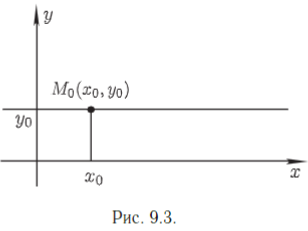
\includegraphics{C:/Users/dmitr/Documents/Система связи на квантовой запутанности/Система связи на квантовой запутанности/markdown/Мат.анализ/Картинки/Рис.9.3.png}\\
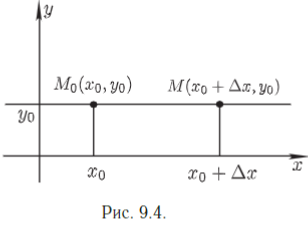
\includegraphics{C:/Users/dmitr/Documents/Система связи на квантовой запутанности/Система связи на квантовой запутанности/markdown/Мат.анализ/Картинки/Рис.9.4.png}

\emph{Определение}. Функция \$u=f(x,y)\$ называется непрерывной в точке
\$M\_0(x\_0,y\_0)\$ по переменной x, если
\$\textbackslash lim\_\{\textbackslash Delta x \textbackslash to 0\}
\textbackslash Delta\_x u = 0\$.

Аналогично определяется непрерывность функции \$u=f(x\_1,...,x\_m)\$ в
данной точке по отдельным переменным.\\
Непрерывность функции, определённую условием (9.2) (или 9.3), называют
также \emph{непрерывность} по совокупности переменных.

\emph{Теорема 6}. Если функция \$u=f(x,y)\$ определена в окрестности
точки \$M\_0(x\_0,y\_0)\$ и непрерывна в точке \$M\_0\$, то она
непрерывна в этой точке по отдельным переменным.\\
\emph{Доказательство}. По условию
\$\textbackslash lim\emph{\{x\textbackslash to x\_0 \textbackslash{}
y\textbackslash to y\_0\} f(x,y) = f(x\_0,y\_0)\$. В частности,
\$\textbackslash lim}\{x\textbackslash to x\_0\} f(x,y\_0) =
f(x\_0,y\_0)\$, а это означает, что \$f(x,y)\$ непрерывна в точке
\$M\_0\$ по переменной x. Аналогично доказывается непрерывность в точке
\$M\_0\$ по переменной y.\\
\emph{Замечание}. Обратное к теореме 6 утверждение не верно.

\hypertarget{ux43eux441ux43dux43eux432ux43dux44bux435-ux442ux435ux43eux440ux435ux43cux44b-ux43e-ux43dux435ux43fux440ux435ux440ux44bux432ux43dux44bux445-ux444ux443ux43dux43aux446ux438ux44fux445}{%
\subsection{Основные теоремы о непрерывных
функциях}\label{ux43eux441ux43dux43eux432ux43dux44bux435-ux442ux435ux43eux440ux435ux43cux44b-ux43e-ux43dux435ux43fux440ux435ux440ux44bux432ux43dux44bux445-ux444ux443ux43dux43aux446ux438ux44fux445}}

Теорема 7 (арифметические операции над непрерывными функциями). Если
функции \$f(M)\$ и \$g(M)\$ определены на множестве \$\{ M\}\$ и
непрерывны в точке A, то \$f(M)\textbackslash plusmn g(M)\$,
\$f(M)g(M)\$, \$\textbackslash frac\{f(M)\}\{g(M)\}\$(при условии \$g(A)
\textbackslash neq 0\$) непрерывны в точке A.

Утверждение теоремы 7 следует из теоремы 4 и определения непрерывности.

Пусть аргументы функции \$u =f(x\_1,....,x\_m)\$ являются не
независимыми переменными, а функциями переменных \$t\_1,...,t\_k\$:

\[x_1 = \phi_1(t_1,...,t_k),...,x_m = \phi_m(t_1,...,t_k) (9.4)\]

причем функции (9.4) определены на множестве
\$\{\textbackslash mathbb\{K\}(t\_1,...t\_k)\} \textbackslash subset
\textbackslash R\^{}k\$.\\
В этом случае будем говорить что на множестве
\$\{\textbackslash mathbb\{K\}\}\$ определена \emph{сложная функция}
\$u=f(\textbackslash phi(t\_1,...,t\_k)),...,\textbackslash phi\_m(t\_1,...,t\_k)\$).\\
\emph{Теорема 8} (о непрерывности сложной функции). Пусть функции (9.4)
непрерывны в точке \$A (a\_1,...a\_k)\$, а функция
\$u=f(x\_1,...,x\_m)\$ непрерывна в точке \$B(b\_1,...,b\_m)\$. где
\$b\_1 = \textbackslash phi\_1(a\_1,...,a\_k),...,b\_m
=\textbackslash phi\_m(a\_1,...,a\_k)\$. Тогда сложная функция
\$u=f(\textbackslash phi\_1(t\_1,...,t\_k),...,\textbackslash phi\_m(t\_1,...t\_k))\$
непрерывна в точке A.

\emph{Теорема 9} (об устойчивости знака непрерывной функции).\\
Если функция \$u=f(M)\$ непрерывна в точке \$A\$ и \$f(A) \textgreater{}
0\$(\textless0), то \$\textbackslash exist \textbackslash delta\$-
окрестность точки A, в которой\\
\$f(M)\textgreater0(\textless0)\$.\\
Указание: для доказательства теоремы воспользуйтесь определением
непрерывности функции в точке A и возьмите
\$\textbackslash epsilon=\textbar f(A)\textbar\$.

\emph{Теорема 10} (о прохождении непрерывной функции через любое
промежуточное значение). Пусть функция \$u=f(M)=f(x\_1,...,x\_m)\$
непрерывна на связном множестве \$\{M\}\$, пусть \$M\_1\$ и \$M\_2\$ -
две любые точки из \$\{M\}\$, \$f(M\_1) = u\_1\$, \$f(M\_2) = u\_2\$, и
пусть \$u\_0\$- любое число из сегмента \${[}u\_1,u\_2{]}\$.\\
Тогда из любой непрерывной кривой \$L\$, соединяющей точки\\
\$M\_1\$ и \$M\_2\$ и целиком принадлежащей множеству \$\{M\}\$,
найдется такая точка \$M\_0\$, такая, что \$f(M\_0)=u\_0\$.\\
\emph{Доказательство}. Пусть

\[L=\{M(x_1,...,x_m):x_1=\phi_1(t),...,x_m=\phi_m(t),\alpha \leq t \leq \beta\}
$$- непрерывная кривая, соединяющая точки $M_1$ и $M_2$ и целиком принадлежащая множеству $\{M\}$ (рис. 9.5).

Точки $M_1$ и $M_2$ имеют координаты: $M_1(\phi_1(\alpha),...,\phi_m(\alpha))$, $M_2(\phi_1(\Beta),...,\phi_m(\Beta))$.

На кривой L заданная функция является сложной функцией переменной t:\]

\begin{Shaded}
\begin{Highlighting}[]
\NormalTok{u=f(\textbackslash{}phi\_1(t),...,\textbackslash{}phi\_m(t))=:F(t)}
\end{Highlighting}
\end{Shaded}

\$\$,\\
причем по теореме 8 функция \$F(t)\$ непрерывная на сегменте
\${[}\textbackslash alpha,\textbackslash beta{]}\$. На концах сегмента
\${[}\textbackslash alpha,\textbackslash beta{]}\$ функция \$F(t)\$
имеет значения \$F(\textbackslash alpha) =
f(\textbackslash phi\_1(\textbackslash alpha),...,\textbackslash phi\_m(\textbackslash alpha))=f(M\_1)=u\_1\$
и \$F(\textbackslash beta) = f(M\_2) = u\_2\$.\\
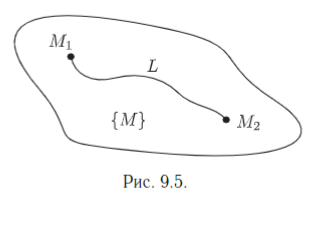
\includegraphics{C:/Users/dmitr/Documents/Система связи на квантовой запутанности/Система связи на квантовой запутанности/markdown/Мат.анализ/Картинки/Рис.9.5.png}

В силу известной теоремы для функции одной переменной \\
\$\textbackslash forall u\_0 \textbackslash in {[}u\_1,u\_2{]}
\textbackslash exist t\_0 \textbackslash in
{[}\textbackslash alpha,\textbackslash beta{]}\$, такое, что \$F(t\_0) =
u\_0\$. Но \$F(t\_0) =
f(\textbackslash phi\_1(t\_0),...,\textbackslash phi\_m(t\_0)) =
f(M\_0)\$, причем точка
\$M\_0(\textbackslash phi\_1(t\_0),...,\textbackslash phi\_m(t\_0))\textbackslash in
L\$.

Итак, \$\textbackslash exist\$ точка \$M\_0 \textbackslash in L: f(M\_0)
= u\_0\$, что и требовалось доказать.\\
Для доказательства следующих трёх теорем (первой и второй теорем
Вейерштрасса и теоремы Кантора) нам понадобится\\
\emph{Лемма 3}. Пусть \{\$M\$\} - замкнутое множество и пусть
последовательность точек \{\$M\_n\$\} \$\textbackslash to\$ \$A\$,
причем все \$M\_n \textbackslash in\$\{\$M\$\}. Тогда \$A
\textbackslash in \{ M\}\$.\\
\emph{Доказательство}. Так, как \{\$M\_n\$\} \$\textbackslash to A\$, то
в любой \$\textbackslash epsilon\$ - окрестности точки A содержатся
члены последовательности \{\$M\_n\$\}. Тем самым, в любой
\$\textbackslash epsilon\$-окрестности точки A содержатся точки из
множества \{\$M\$\}. Поэтому точка A - либо внутренняя точка множества
\{\$M\$\}, и тогда она принадлежит этому множеству как и всякая
внутренняя точка, либо \$A\$- граничная точка множества \{\$M\$\}, и
тогда она принадлежит \{\$M\$\}, так как множество \{\$M\$\} - замкнутое
множество (то есть содержит все свои граничные точки). Таким образом, в
любом случае \$A\textbackslash in \{M\}\$. Лемма 3 доказана.\\
\emph{Замечание}. Это утверждение аналогично следующему утверждению для
одномерного случая: если все \$x\_n \textbackslash in {[}a,b{]}\$ и
\{\$x\_n\$\} \$\textbackslash to \textbackslash epsilon\$, то
\$\textbackslash epsilon \textbackslash in {[}a,b{]}\$.

\emph{Определение}. Функция \$u=f(M)\$ называется \emph{ограниченной} на
множестве \$\{M\}\$, если \$\textbackslash exist\$ числа \$C\_1 и
C\_2\$, такие, что \$\textbackslash forall M \textbackslash in
\{M\}:C\_1 \textbackslash leq f(M) \textbackslash leq C\_2\$.

\emph{Теорема 11} (первая теорема Вейерштрасса). Если функция \$u=f(M)\$
непрерывна на \emph{замкнутом ограниченном} множестве \{M\}, то она
ограничена на этом множестве.

\emph{Доказательство}. Допустим, что \$u=f(M)\$ не ограничена на
множестве \{\$M\$\}. Тогда \$\textbackslash forall\$ натурального числа
n\$\textbackslash exist M\_n \textbackslash in
\{\$M\$\}:\textbar f(M\_n)\textbar{} \textgreater{} n\$. Тем самым
последовательность \{\$f(M\_n)\$\} - бесконечно большая. Из ограниченной
последовательности точек \{\$M\_n\$\} можно выделить сходящуюся
подпоследовательность. Пусть подпоследовательность
\{\$M\emph{\{k\_n\}\$\} \$\textbackslash to A\$. В силу леммы 3 точка
\$A \textbackslash in \{M\}\$ и поэтому функция \$f(M)\$ непрерывна в
точке A. Следовательно, \{f(M}\{k\_n\})\} \$\textbackslash to f(A)\$, а
это противоречит тому, что \{\$f(M\emph{\{k\_n\})\$\} -бесконечно
большая последовательность.\\
Полученное противоречие доказывает, что наше предположение не верно и,
следовательно, функция \$u=f(M)\$ ограниченна на множестве \{\$M\$\}.\\
\_Замечание}. Если множество \{\$M\$\} не является ограниченным или не
является замкнутым, то непрерывная на таком множестве функция \$u=f(M)\$
может быть неограниченной на этом множестве.

\emph{Определение}. Число U называется \emph{точной верхней гранью}
функции \$u=f(M)\$ на множестве \{\$M\$\}, если \\
1: \$\textbackslash forall M \textbackslash in \{ M\}:f(M)
\textbackslash leq U\$;\\
2: \$\textbackslash forall\textbackslash{} числа\textbackslash{}
\textbackslash widetilde\{U\}\textless U\textbackslash exist
\textbackslash widetilde\{M\} \textbackslash in
\{M\}:f(\textbackslash widetilde\{M\}) \textgreater{}
\textbackslash widetilde\{U\}\$.\\
\emph{Обозначение}: U = \textbackslash sup\emph{\{\{M\}\}f(M),\\
Аналогично определяется точная нижняя грань функции
\$\textbackslash int}\{\{M\}\}f(M)\$.

\emph{Теорема 12} (вторая теорема Вейерштрасса). Непрерывная на
замкнутом ограниченном множестве функция достигает на этом множестве
своих точных нижней и верхней граней.

Теорема доказывается так же, как и аналогичная теорема для функции одной
переменной.

\emph{Определение}. Функция \$u=f(M)\$ называется \emph{равномерно
непрерывной} на множестве \{\$M\$\}, если \$\textbackslash forall
\textbackslash epsilon \textgreater{} 0 \textbackslash exist
\textbackslash delta \textgreater0\$(зависящее только от
\$\textbackslash epsilon\$), такое, что \$\textbackslash forall M\_1\$ и
\$M\_2\$ из множества \{\$M\$\}, удовлетворяющих условию
\$\textbackslash rho(M\_1,M\_2)\textless\textbackslash delta\$,
выполняется неравенство

\[|f(M_1) - f(M_2)| < \epsilon.\]

Теорема 13 (Кантора) Непрерывная на замкнутом ограниченном множестве
функция равномерно непрерывна на этом множестве.\\
Теорема доказывается так же, как и для функции одной переменной.

\end{document}
